\documentclass[xcolor=dvipsnames,hyperref={pdfpagelabels=false}]{beamer}

\usetheme{Boadilla}

\newcommand{\bi}{\begin{itemize}}
\newcommand{\ei}{\end{itemize}}
\newcommand{\be}{\begin{enumerate}}
\newcommand{\ee}{\end{enumerate}}
\newcommand{\bc}{\begin{center}}
\newcommand{\ec}{\end{center}}
\newcommand{\bd}{\begin{description}}
\newcommand{\ed}{\end{description}}
\newcommand{\I}{\item}
\newcommand{\f}{\frame}
\newcommand{\ft}{\frametitle}

\title{Offline Software Overview}
\subtitle{GlueX Collaboration Meeting}
\author[Mark Ito]{Mark M.\ Ito}
\date{October 9, 2015}
\institute[JLab]{Jefferson Lab}

\begin{document}

\f{\titlepage}

\f{\ft{Topics for Following Talks}
\bi
\I Offline Monitoring: Kei
\I Conversion to Geant4: Richard
\I Overhaul ROOT TTree Format: Paul M.
\ei
}

\f{\ft{New Offline Software Wiki Page}

\begin{columns}
\begin{column}{2.0in}
\small
\be
\I General Information
\I Software Documentation
\I Offline Data Monitoring
\I Computing Facilities
\I Software Management
\I Meetings and Reviews
\I Communication and Help
\I Legacy Links
\I Uncategorized Links
\ee
\end{column}
\begin{column}{2.5in}
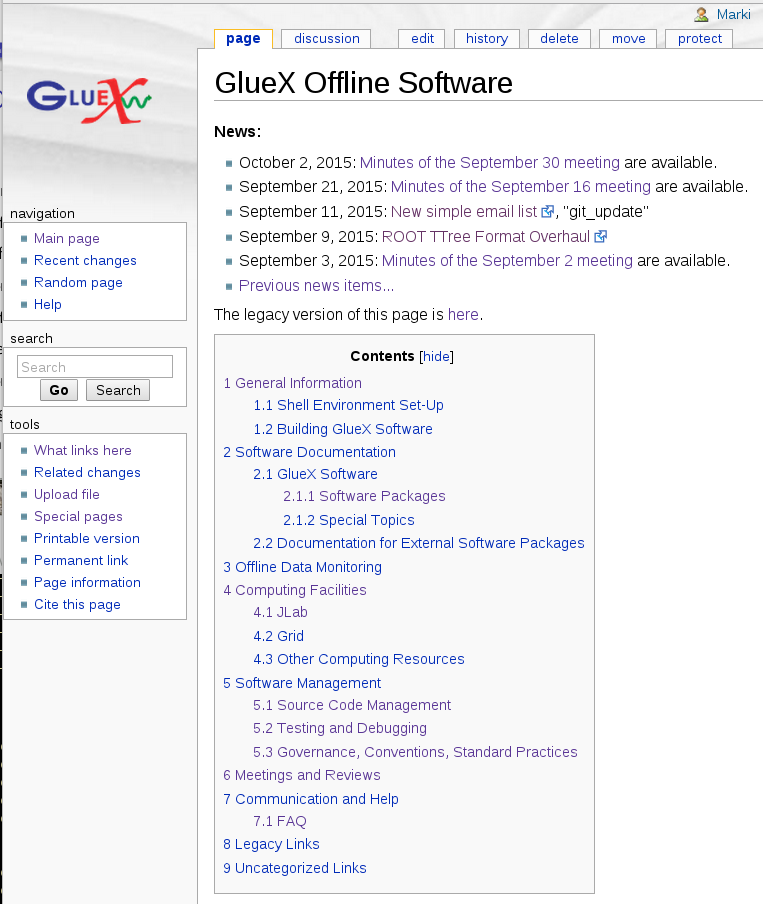
\includegraphics[width=2.4in]{offline_wiki_3.png}
\end{column}
\end{columns}
}

\f{\ft{Conversion to Git}

Director's Review of 12 GeV Software Computing, June~7-8,~2012, Committee Recommendations:

...

17.\ While we encourage the move to git as a code management system, be sure not to underestimate the extent of the paradigm shift. Identify a workflow model for your use of git. Communicate clearly the new paradigm (easy branching, no central repository, etc.). Set up (or link to) tutorials for users with a mapping of routine CVS tasks to their git equivalents (such as cvs diff, etc.). Document or link to documentation for standard git tasks without obvious equivalent in CVS or SVN, such as git rebase, or bisect.

...
}

\f{\ft{Why Change?}
  \bi
  \I Better management of changes
  \I Better communication of changes
  \I Better documentation of changes
  \I Less down-time with broken code on trunk
  \ei
}

\f{\ft{Repositories on GitHub}
  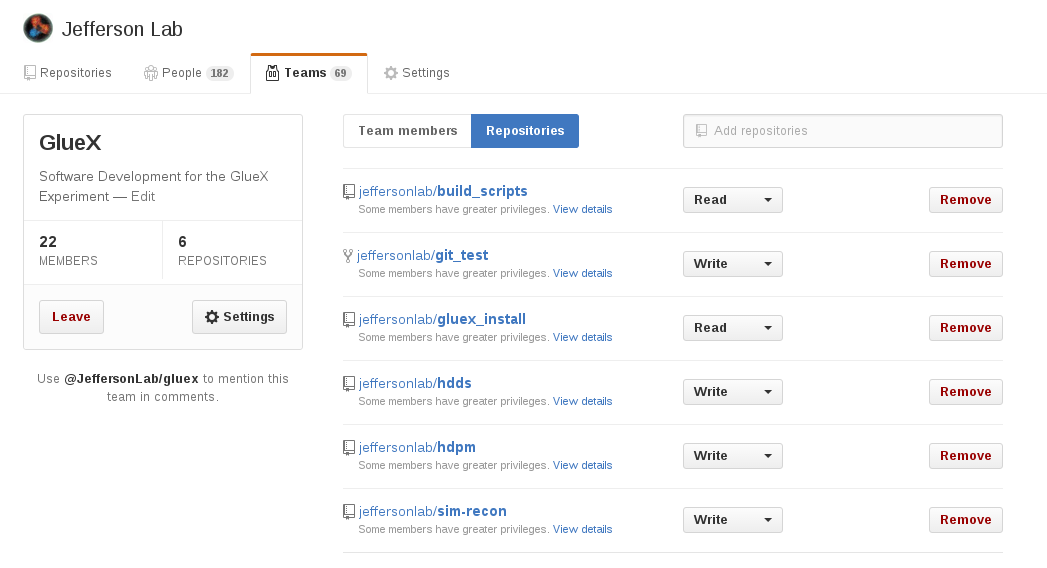
\includegraphics[width=4.5in]{repositories.png}
  }

\f{\ft{Notes on Git/GitHub}
  \bi
  \I Everyone needs an account on GitHub.
  \I Anyone can update the master branch.
  \I Changes should go onto topic branches, but enforced only administratively.
  \I Nightly builds working from the Git Repositories
  \I ``git\_update'' simple email list: daily digest of changes
  \I Team Maintainers and Team Administrators
  \ei
}

\f{\ft{Spring 2015 Simulations Complete}
\bi
\I 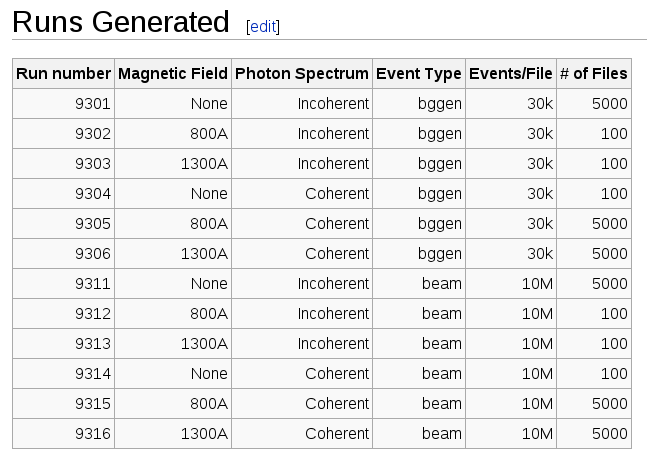
\includegraphics[width=3.5in]{spring_sim_conditions.png}
\I Used sim-recon-1.3.0
\I Run 9306 redone with sim-recon-1.5.1 (BCAL ``raw'' data generated)
\ei
}

\f{\ft{Future Simulation Runs (from Sean)}

\bi
\I new naming scheme, the next effort will be ``sim1''
\I the current state of thinking:
  \bi
  \I use the "mc\_sim1" variation and run 9001
  \I 1350A solenoid field that we decided was the default
  \I For EM background, will the nominal BGRATE=1.1
  \ei
\ei
}

\f{\ft{Hall D Package Manager (HDPM) from Nathan Sparks}
$$
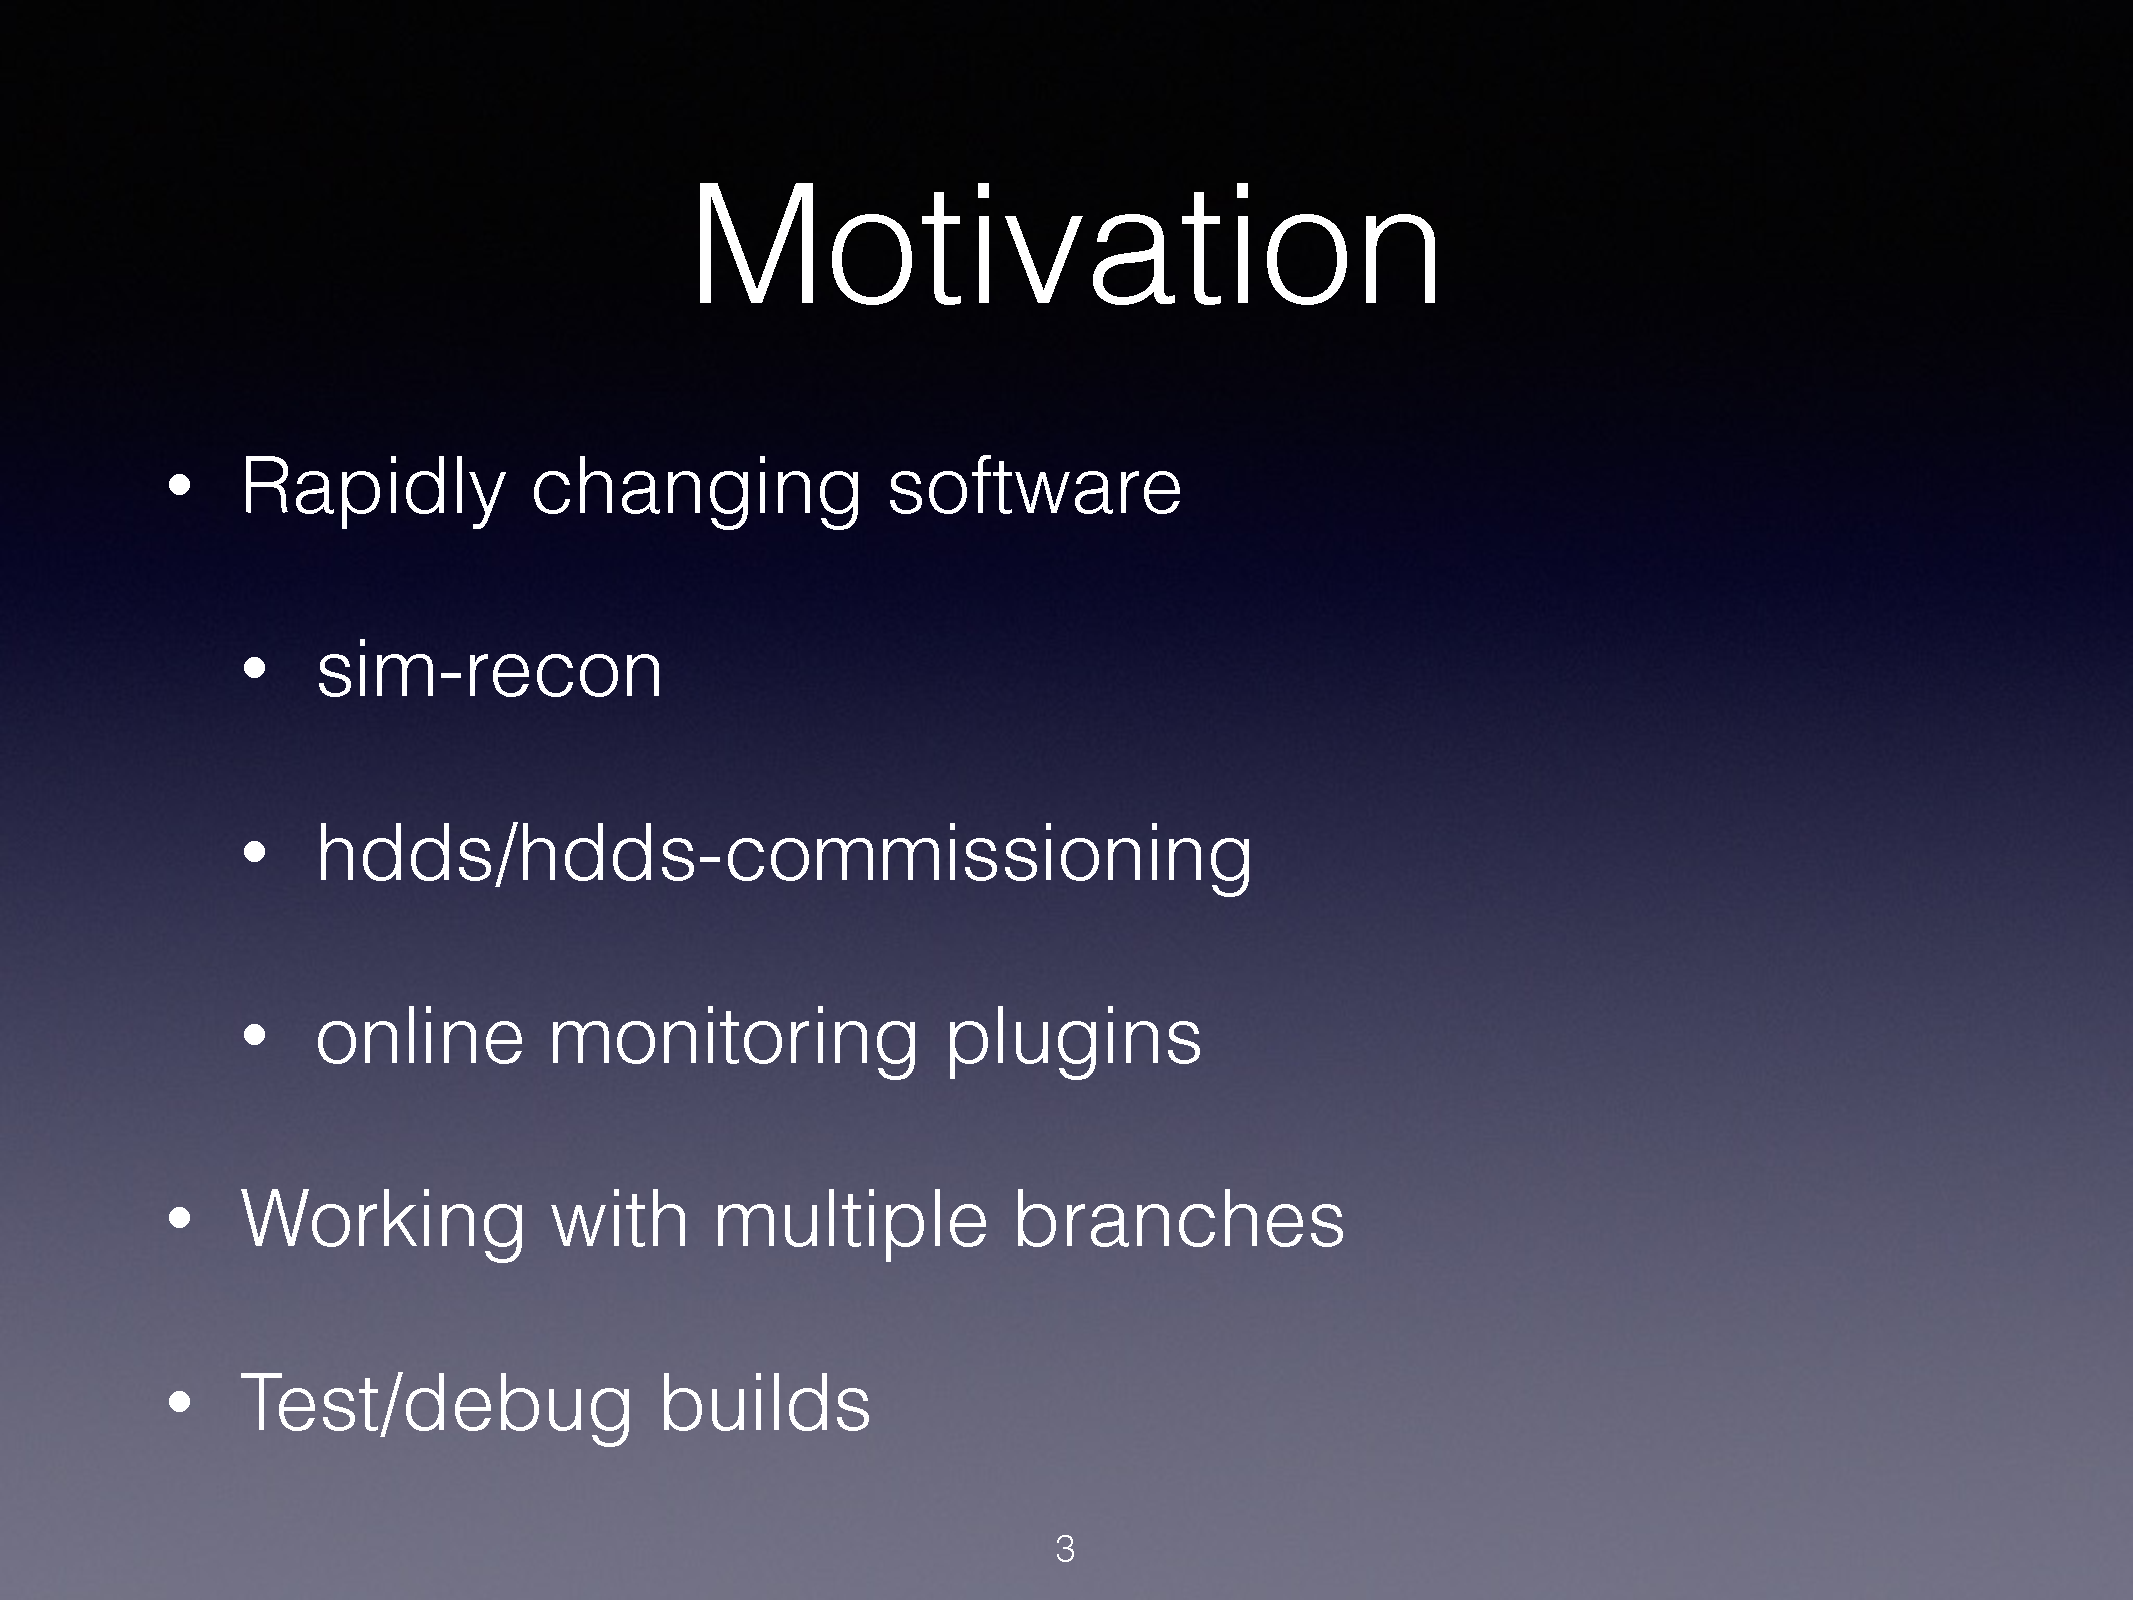
\includegraphics[width=4.0in]{hdpm_motivation.pdf}
$$}

\f{
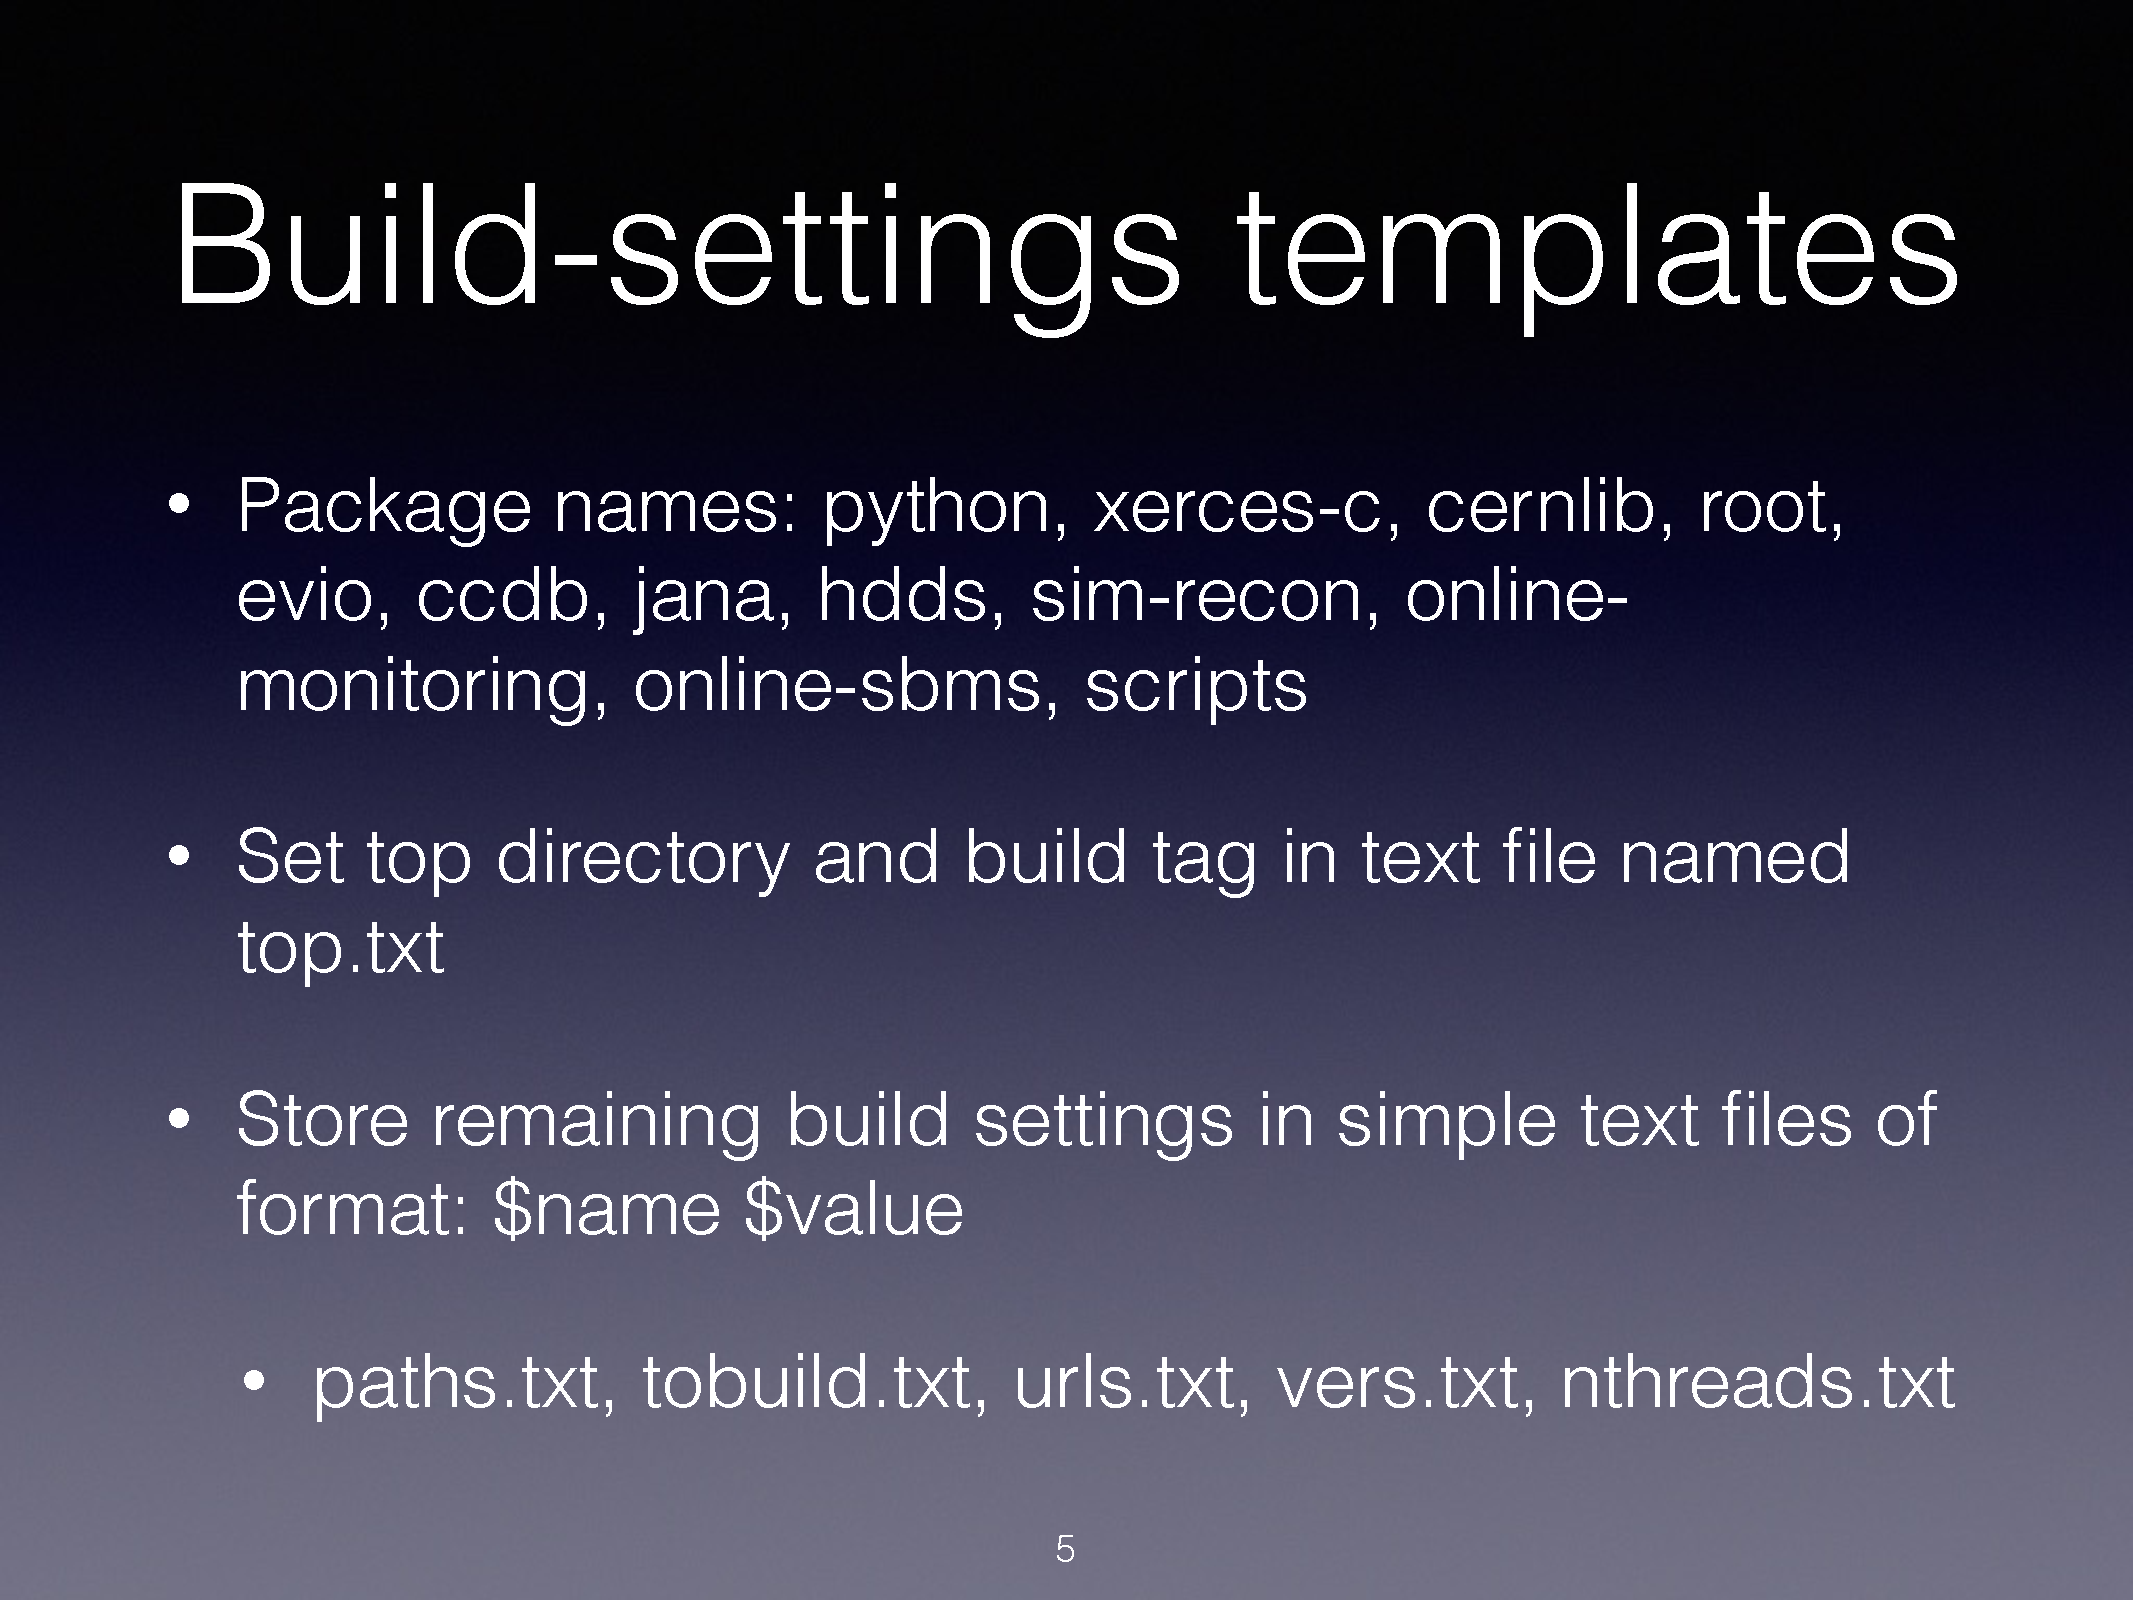
\includegraphics[width=4.5in]{hdpm_templates.pdf}
}

\begin{frame}[fragile]
\scriptsize
settings-Sp15/top.txt:
\begin{verbatim}
# top   build-tag
default Sp15
\end{verbatim}
settings-Sp15/vers.txt:
\begin{verbatim}
xerces-c  3.1.2
cernlib   2005	
root      5.34.26
evio      4.3.1
ccdb      1.05
jana      0.7.3
hdds      latest
sim-recon latest
\end{verbatim}
settings-Sp15/commands.txt:
\begin{verbatim}
hdds      "scons -u install"
sim-recon "scons -u -j8 install"
\end{verbatim}
\end{frame}

\begin{frame}[fragile]
\scriptsize
settings-Sp15/paths.txt:
\begin{verbatim}
xerces-c  /group/halld/Software/builds/[OS]/xerces-c/xerces-c-[VER]
cernlib   /group/halld/Software/builds/[OS]/cernlib
root      /group/halld/Software/builds/[OS]/root/root_[VER]
evio      /group/halld/Software/builds/[OS]/evio/evio-[VER]
ccdb      /group/halld/Software/builds/[OS]/ccdb/ccdb_[VER]
jana      /group/halld/Software/builds/[OS]/jana/jana_[VER]
hdds      hdds
sim-recon sim-recon
\end{verbatim}
settings-Sp15/urls.txt:
\begin{verbatim}
xerces-c  http://www.motorlogy.com/apache/xerces/c/3/sources/xerces-c-[VER].tar.gz
cernlib   http://www-zeuthen.desy.de/linear_collider/cernlib/new/cernlib.2005.corr.2014.04.17.tgz
root      https://root.cern.ch/download/root_v[VER].source.tar.gz
evio      https://coda.jlab.org/drupal/system/files/coda/evio/evio-4.4/evio-[VER].tgz
ccdb      https://github.com/JeffersonLab/ccdb/archive/v[VER].tar.gz
jana      https://www.jlab.org/JANA/releases/jana_[VER].tgz
hdds      https://github.com/JeffersonLab/hdds
sim-recon https://github.com/JeffersonLab/sim-recon
\end{verbatim}
\end{frame}

\f{\ft{Multi-Threaded mcsmear}

David studied the effects. Findings are:

\be
\I HDDM has multiple options for compressing the data stream: no compression, bz2 compression, zlib compression
\I mcsmear runs approximately 3-4 times faster with no compression than with bz2 compression
\I mcsmear does not scale well with multiple threads
  \bi
  \I most of its time is spent in writing the event to the HDDM output stream
  \I this action must be serialized
  \ei
\I Our computing model does not require us to store large amounts of simulated HDDM files on tape
  \bi
  \I if we do, drives have built in compression
  \I cost limited to bandwidth of moving the files to/from tape and local disk storage
  \ei
\ee
}

\f{
\bc
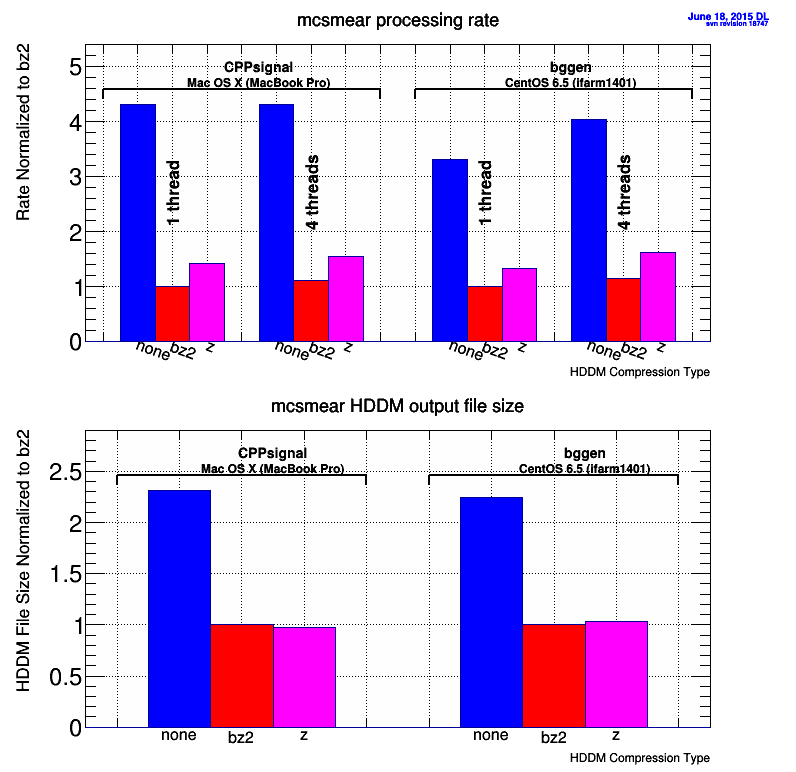
\includegraphics[height=3.0in]{mcsmear_compression.png}
\ec
}

\f{
\bc
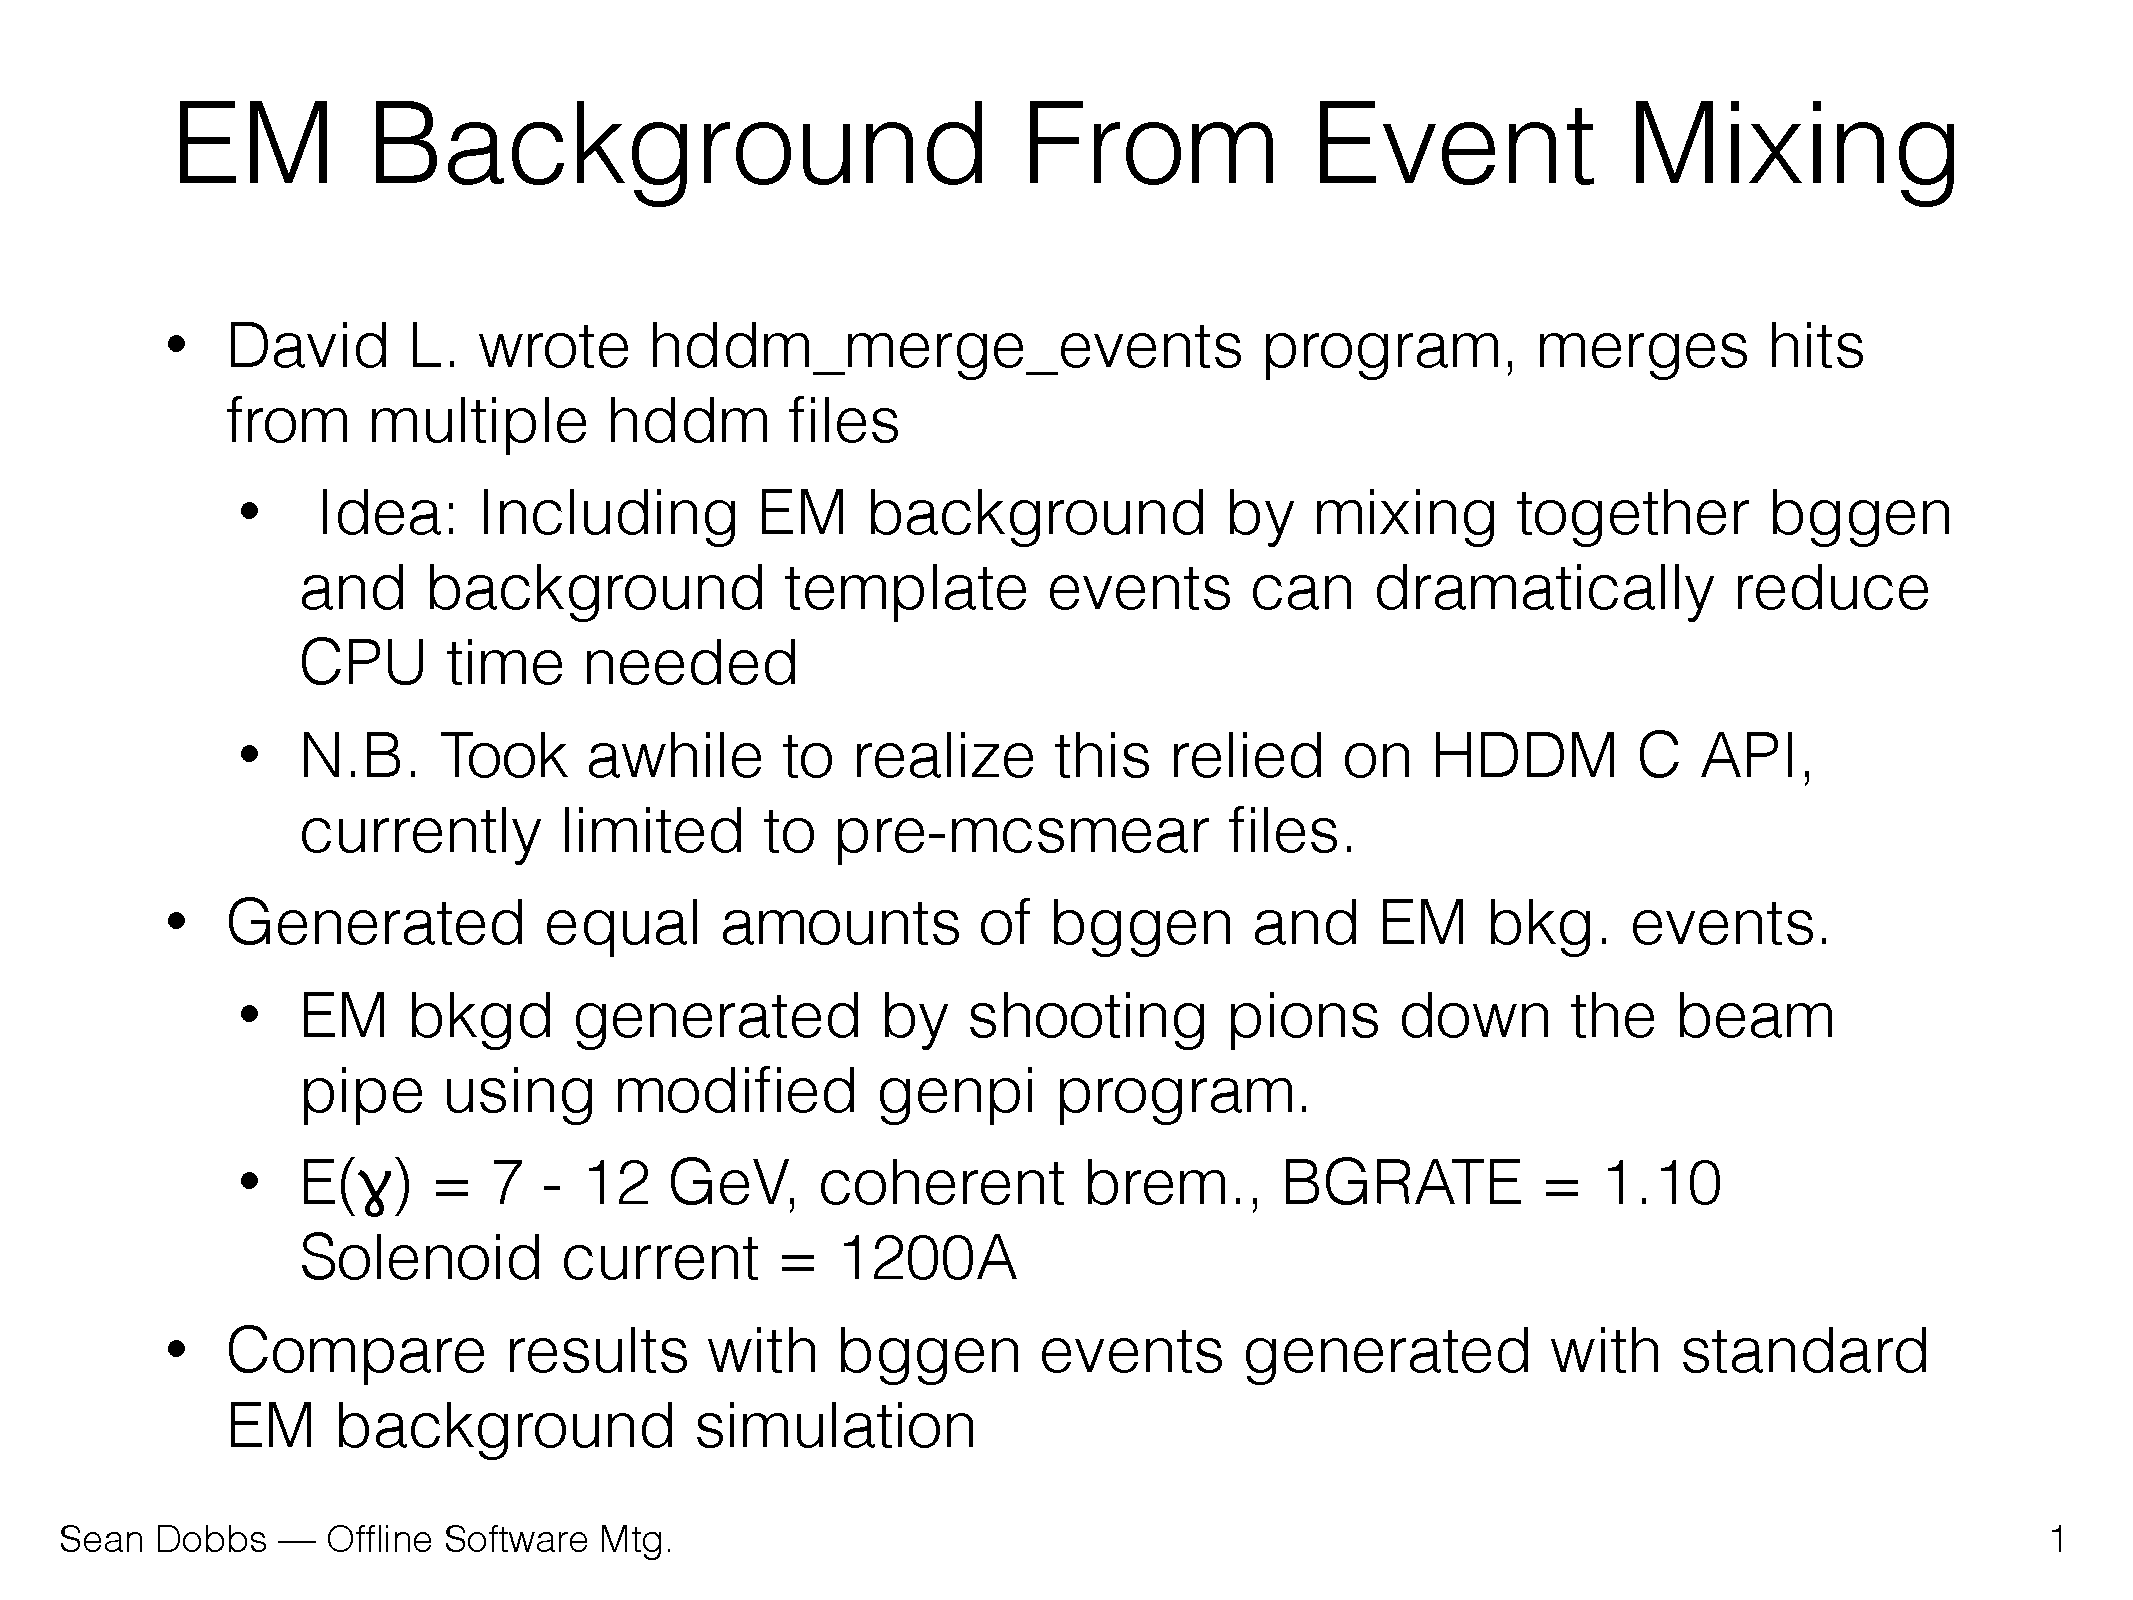
\includegraphics[height=3.0in]{Sdobbs_EMBkgd_1.pdf}
\ec
}

\f{
\bc
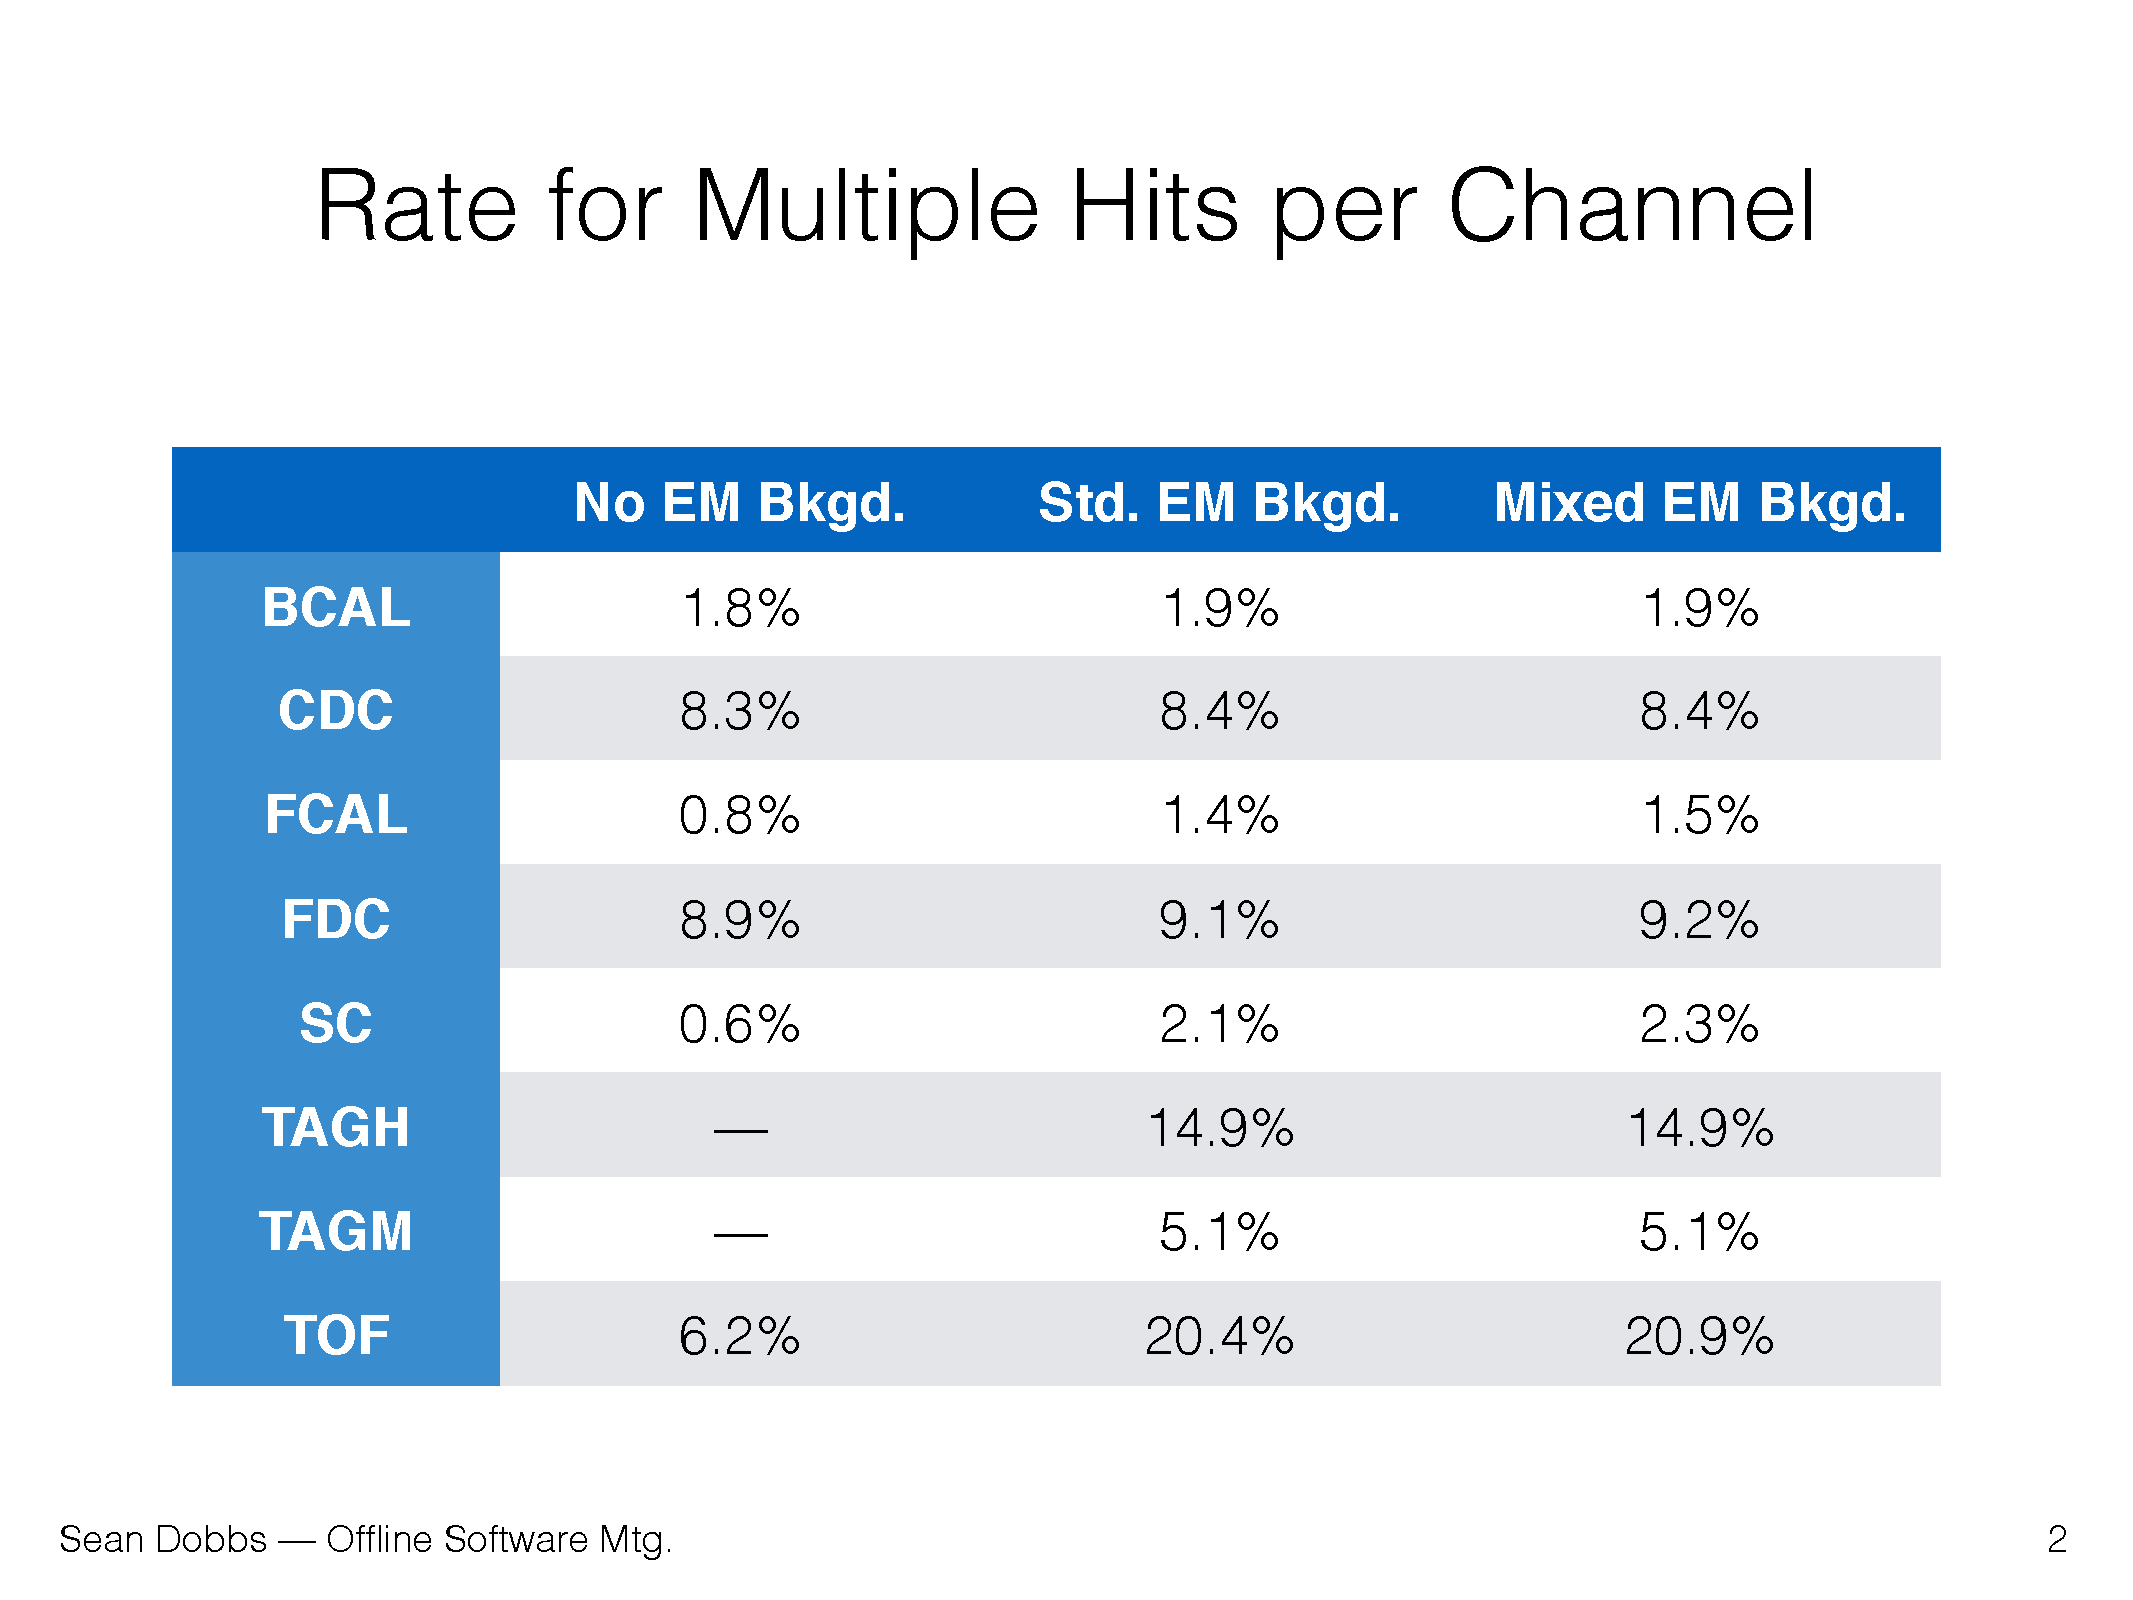
\includegraphics[height=3.0in]{Sdobbs_EMBkgd_2.pdf}
\ec
}

\f{
\bc
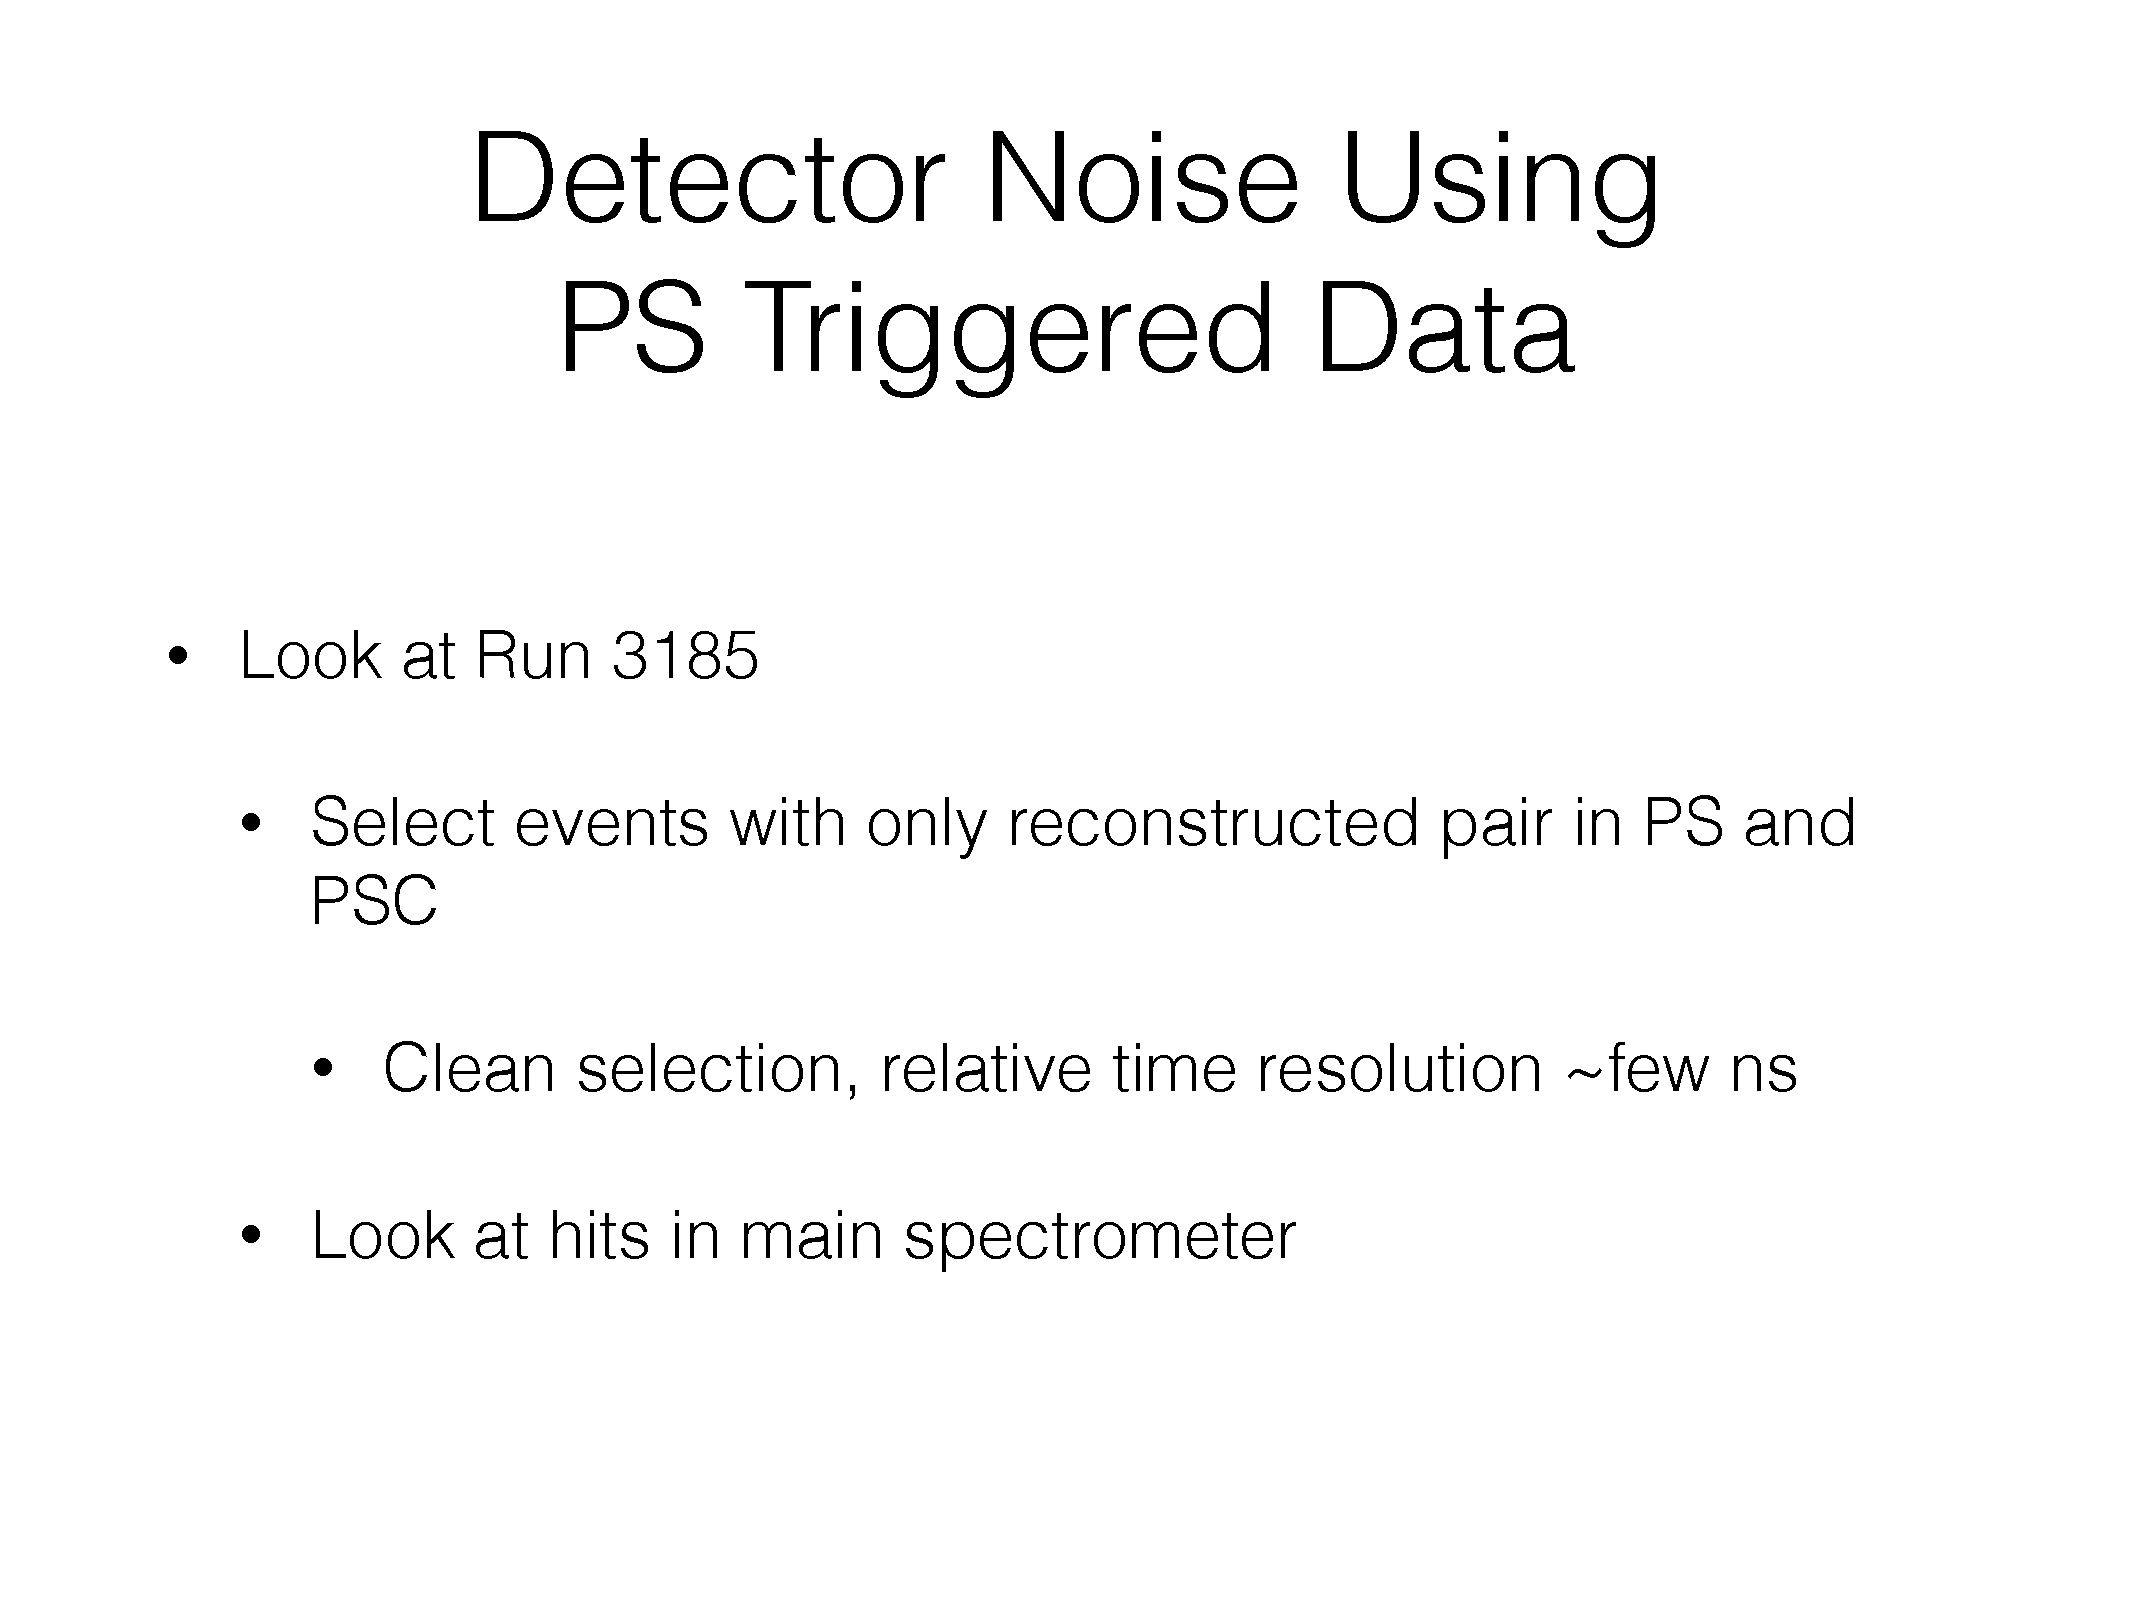
\includegraphics[height=3.0in]{Sdobbs_pstrig_1.pdf}
\ec
}

\f{
\bc
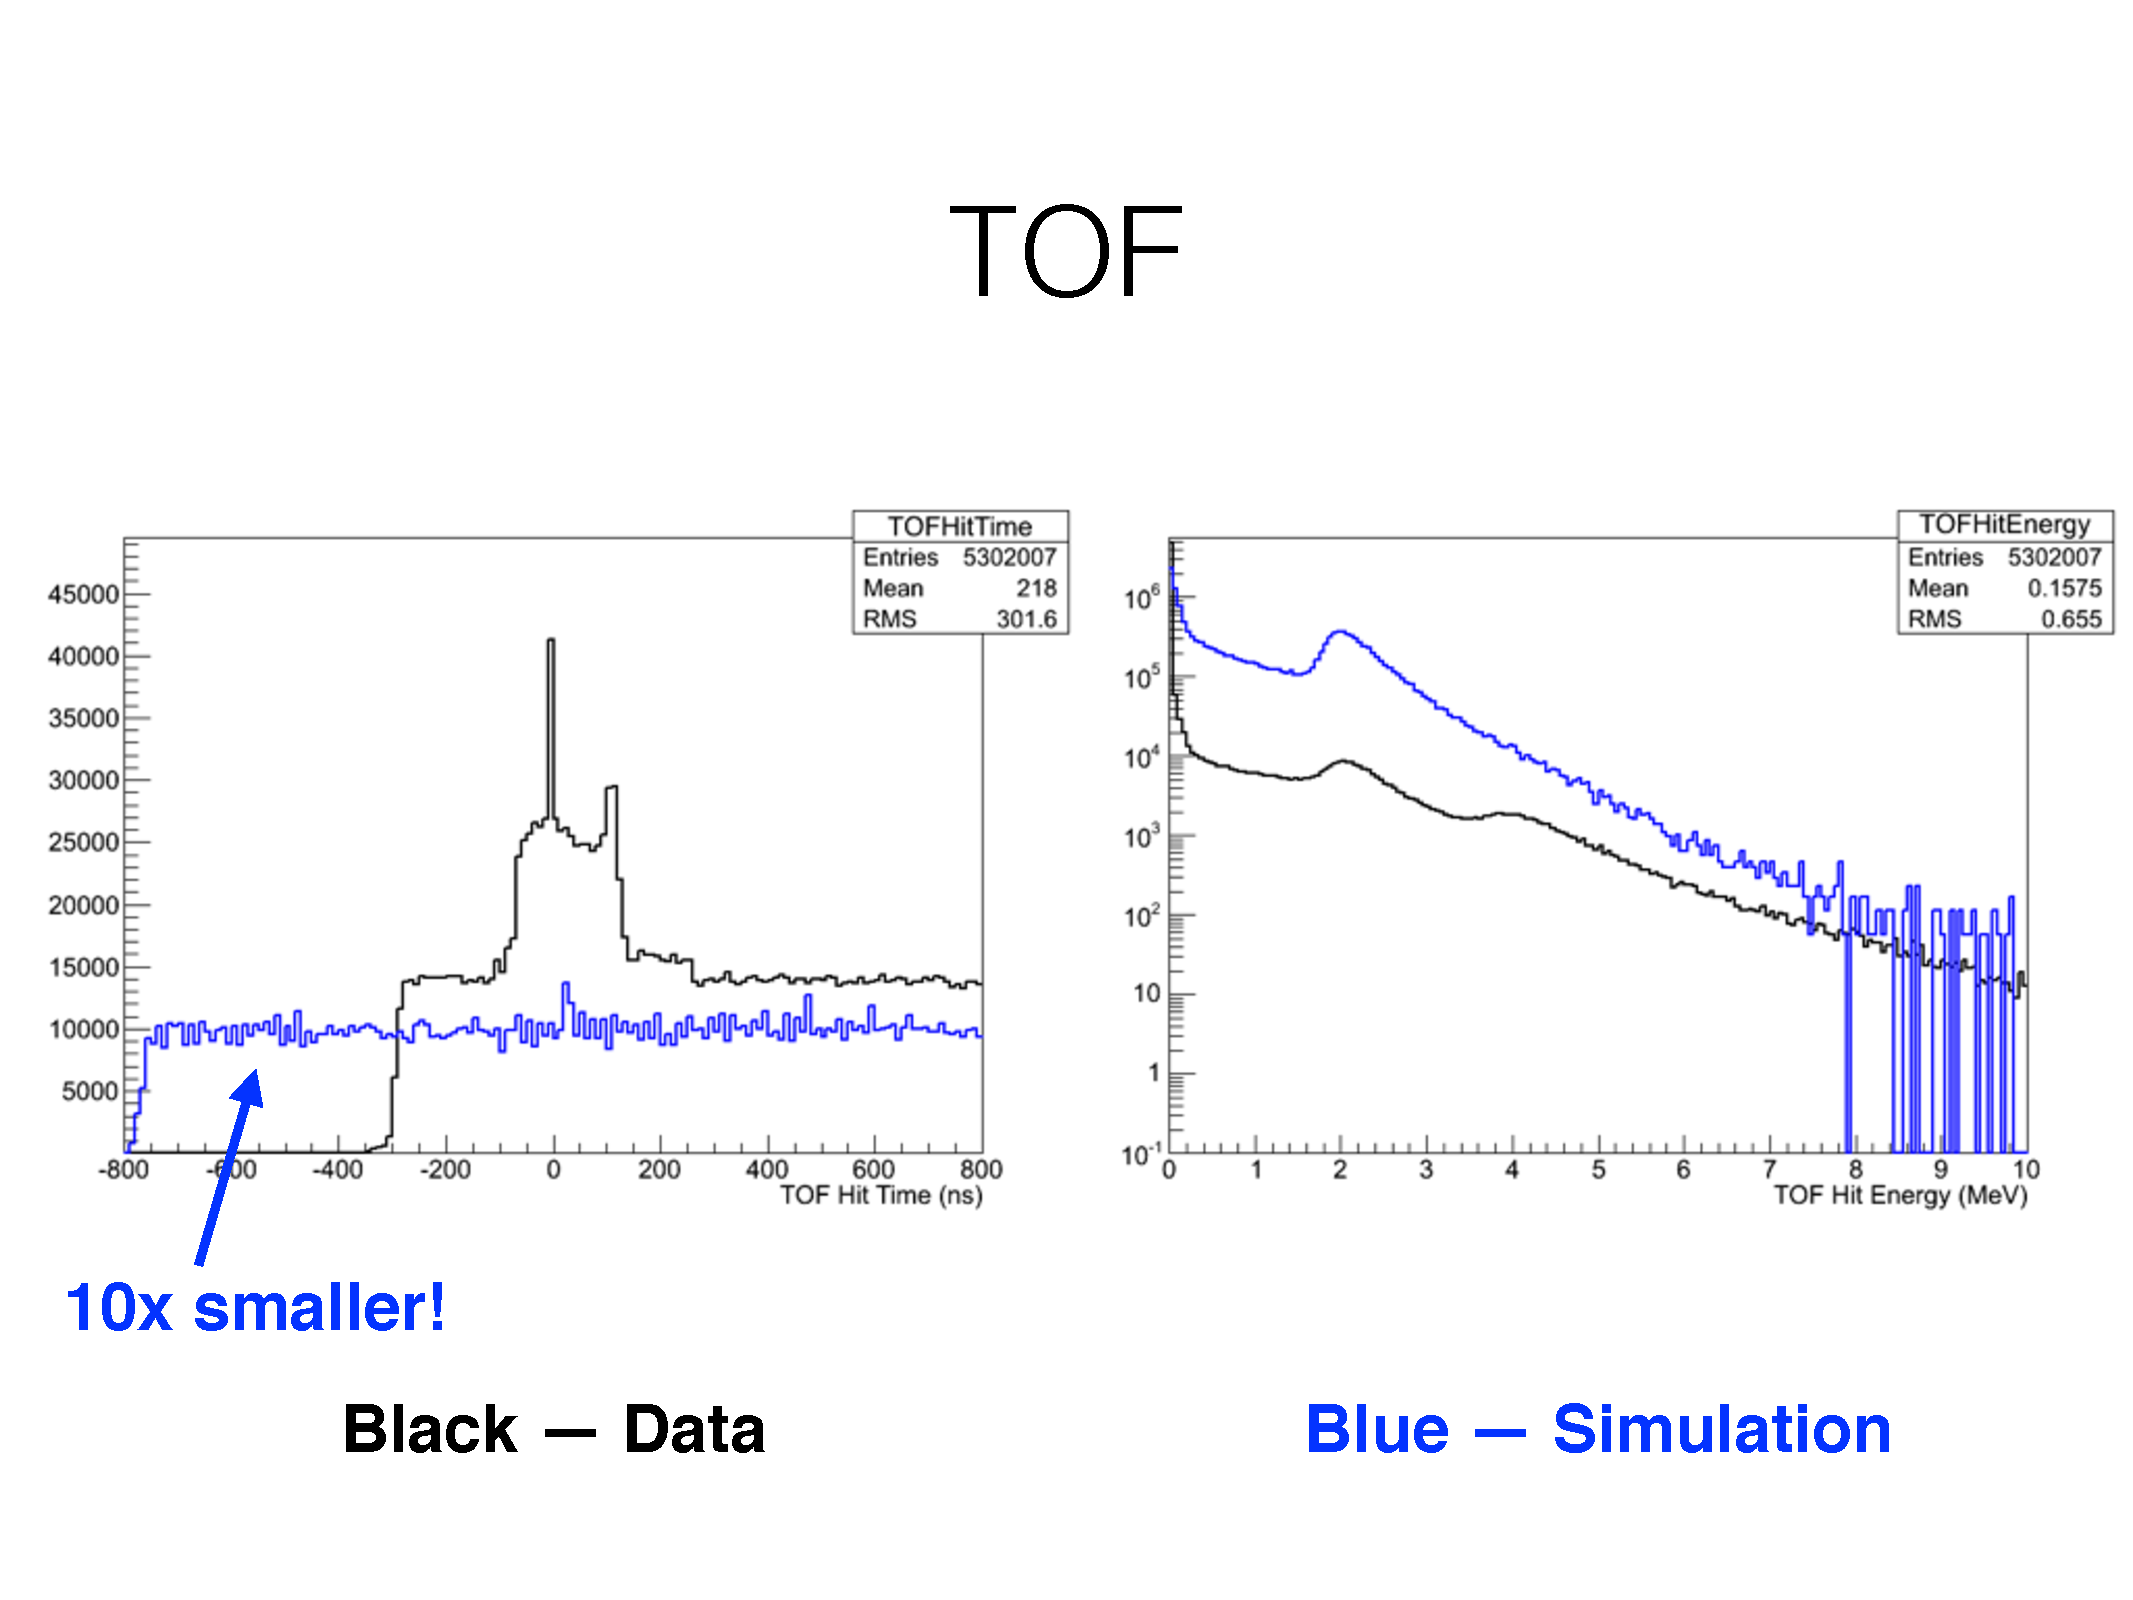
\includegraphics[height=3.0in]{Sdobbs_pstrig_2.pdf}
\ec
}

\f{\ft{New Releases Since the Last Meeting}
\bc
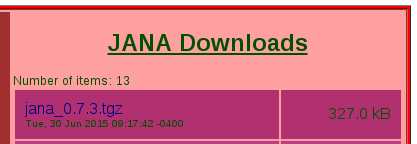
\includegraphics[height=.7in]{jana_releases.png} \\
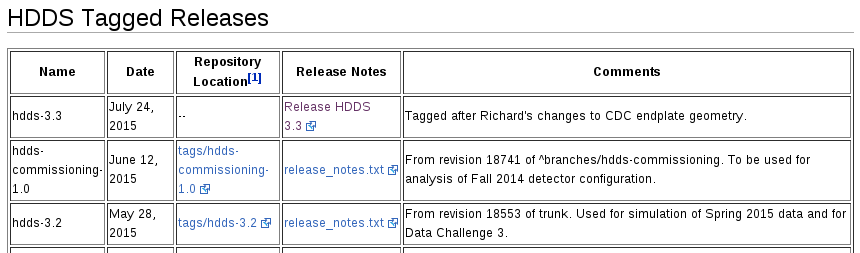
\includegraphics[height=1.0in]{hdds_releases.png} \\
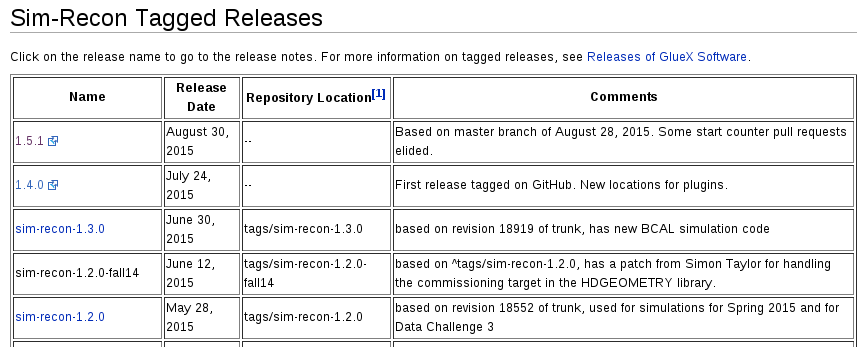
\includegraphics[height=1.5in]{sim-recon_releases.png}
\ec
}

\f{\ft{Other Topics 1}
\bi
\I New volatile disk hardware: upgrade from Lustre 1.8 to 2.5
\I New work disk hardware: traditional fileserver to Lustre
\I Offline style build on gluon cluster: already there on the group disk
\I ROOT 6: Beni demonstrated compatibility, still some work to do
\I Turning the Fine-Mesh Field Map into a Resource: Sean did the work
\I Moving the Plug-Ins from online tree to offline: done by David for use by Offline Monitoring
\I Policy on CCDB Variations for Reconstructing Simulated Data: we have one
\ei
}

\f{\ft{Other Topics 2}
\bi
\I Software for Correcting for Pedestal Drifts: discussion started
\I Data Challenge 3: one pass done, converting to SWIF to streamline tape access
\I Default for builds: with debug symbols or without? Stay with with-symbols
\I F125 algorithms: Mike S. found problem, corrupt times for small pulses
\I Auto-Build on Pull Request: working version in place, almost ready for roll-out
\ei
}

\end{document}
